\chapter[Ordinal Correlation]{Ordinal correlation equals bipolar-valued relational equivalence}
\label{sec:16}

\abstract*{}

\abstract{}

\section{Coping with missing data}
\label{sec:16.1}

In a stubborn keeping with a two-valued logic, where every argument can only be true or false, there is no place for efficiently taking into account missing data or logical indeterminateness. These cases are seen as problematic and, at best are simply ignored. Worst, in modern data science, missing data get often replaced with \emph{fictive} values, potentially falsifying hence all subsequent computations.

In social choice problems like elections, abstentions are, however, frequently observed and represent a social expression that may be significant for revealing non represented social preferences. And, in marketing studies, interviewees will not always respond to all the submitted questions. Again, such abstentions do sometimes contain nevertheless valid information concerning consumer preferences.

Let us consider such a performance tableau in file \texttt{graffiti07.py} \footnote{The file \texttt{graffiti07.py} may be found in the \texttt{examples} directory of the \Digraph resources.} gathering a Movie Magazine's rating of some movies that could actually be seen in town \footnote{\emph{Graffiti}, Edition Revue Luxembourg, September 2007, p. 30. The data file \texttt{graffiti07.py} (\texttt{PerformanceTableau} format) may be found in the \texttt{examples} directory of the \Digraph resources.} (see Fig. \ref{fig:16.1}).
\begin{lstlisting}
>>> from outrankingDigraphs import\
...     PerformanceTableau 
>>> t = PerformanceTableau('graffiti07')
>>> t.showHTMLPerformanceTableau(\
...               title='Graffiti Star wars',\
...               ndigits=0)
\end{lstlisting}
\begin{figure}[h]
%\sidecaption
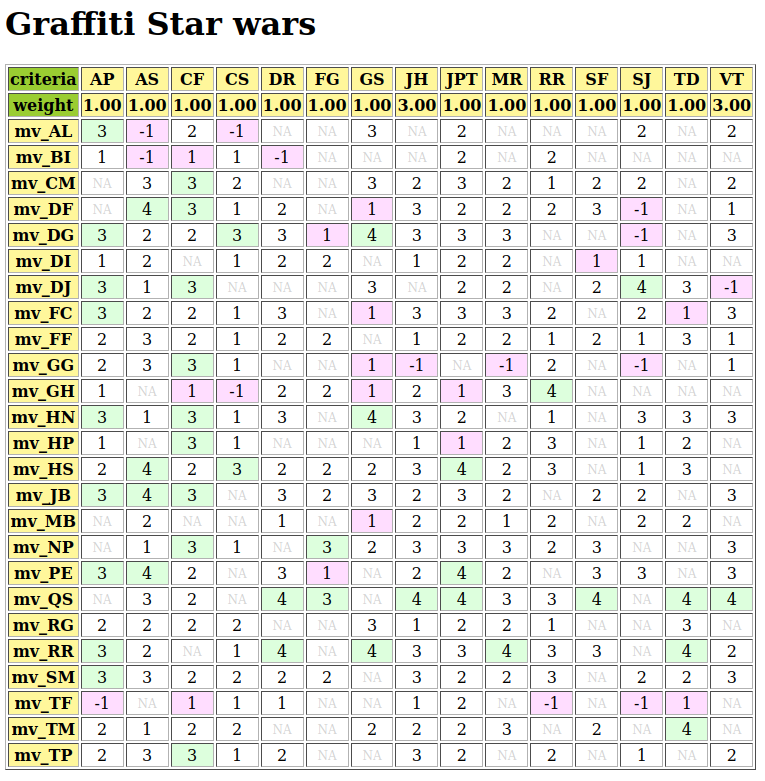
\includegraphics[width=10cm]{Figures/graffiti07_1.png}
\caption{\emph{Graffiti} magazine's movie ratings from September 2007.}
\label{fig:16.1}       % Give a unique label
\end{figure}
15 journalists and movie critics provide here their rating of 25 movies: 5 stars (\emph{masterpiece}), 4 stars (\emph{must be seen}), 3 stars (\emph{excellent}), 2 stars (\emph{good}), 1 star (\emph{could be seen}), -1 star (\emph{I do not like}), -2 (\emph{I hate}), \texttt{NA} (\emph{not seen}).

To aggregate all the critics' rating opinions, the \emph{Graffiti} magazine provides for each movie a global score computed as an average grade, just ignoring the \emph{not seen} data. These averages are thus not computed on comparable denominators; some critics do indeed use a more or less extended range of grades. The movies not seen by critic $SJ$, for instance, are favored, as this critic is more severe than others in her grading. Dropping the movies that were not seen by all the critics is here not possible either, as no one of the 25 movies was actually seen by all the critics. Providing any value for the missing data will as well always somehow falsify any global value scoring. What to do ?

A better approach is to rank the movies on the basis of pairwise bipolar-valued  ``\emph{at least as well rated as}'' opinions. Under this epistemic argumentation approach, missing data are naturally treated as opinion abstentions and hence do not falsify the logical computations. Such a ranking of the 25 movies is provided, for instance, by the \textbf{heatmap} view shown in Fig. \ref{fig:16.2}.

\begin{lstlisting}
>>> t.showHTMLPerformanceHeatmap(\
...                       Correlations=True,\
...                       rankingRule='NetFlows',
...                       ndigits=0)
\end{lstlisting}
\begin{figure}[h]
%\sidecaption
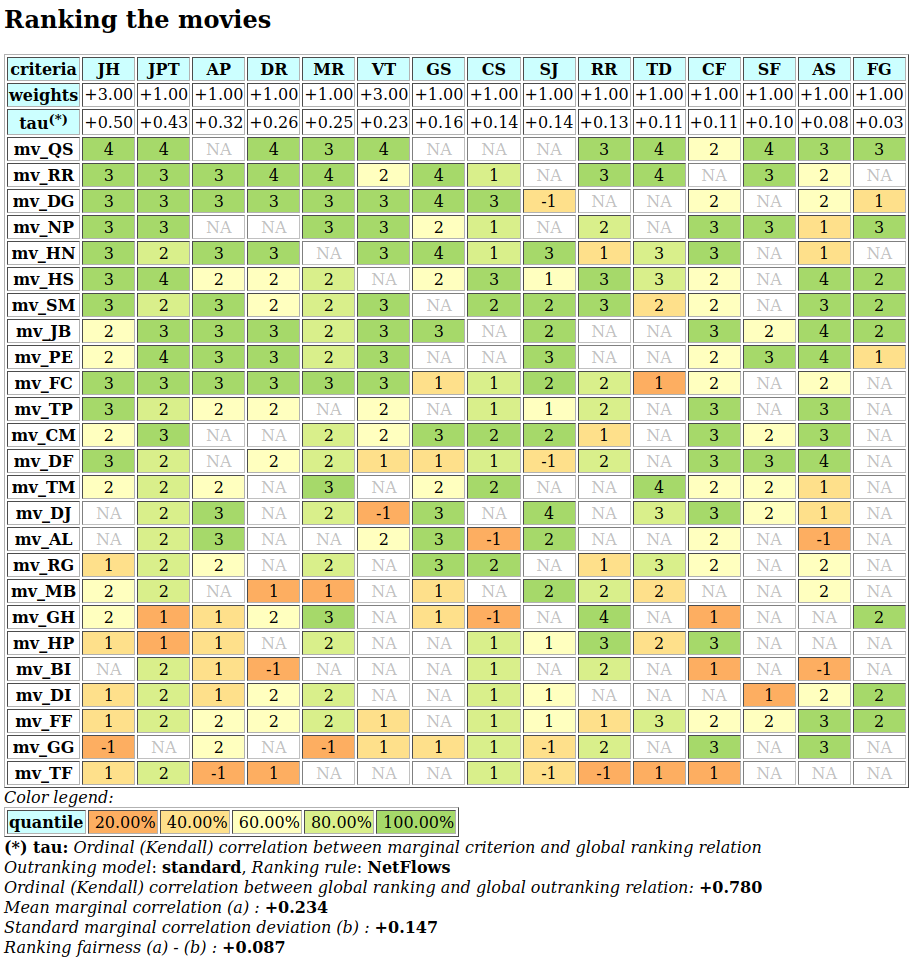
\includegraphics[width=10cm]{Figures/graffiti07_2.png}
\caption{\emph{Graffiti} magazine's ordered movie ratings from September 2007}
\label{fig:16.2}       % Give a unique label
\end{figure}

There is no doubt that movie 'mv\_QS', with 6 \emph{must be seen} marks, is correctly best-ranked and the movie 'mv\_TV' is worst-ranked with five \emph{don't like} marks.

\section{Modelling pairwise bipolar-valued rating opinions}
\label{sec:16.2}

Let us explicitly construct the underlying bipolar-valued outranking digraph and consult in Fig. \ref{fig:16.3} the pairwise characteristic values we observe between the two best-ranked movies, namely 'mv\_QS' and 'mv\_RR'.

\begin{lstlisting}
>>> from outrankingDigraphs import\
...     BipolarOutrankingDigraph
>>> g = BipolarOutrankingDigraph(t)
>>> g.recodeValuation(-19,19) # integer characteristics
>>> g.showHTMLPairwiseOutrankings('mv_QS','mv_RR')
\end{lstlisting}
\begin{figure}[h]
%\sidecaption
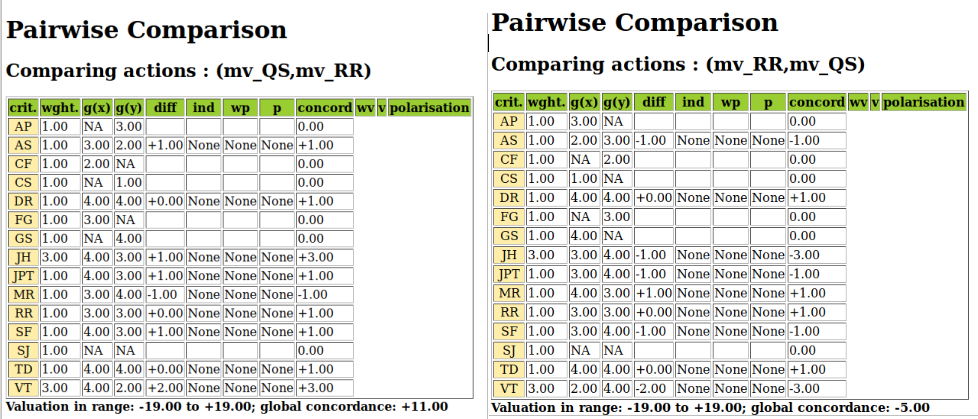
\includegraphics[width=11cm]{Figures/graffiti07_45.png}
\caption{Pairwise comparison of the two best-ranked movies.}
\label{fig:16.3}       % Give a unique label
\end{figure}

Six out of the fifteen critics have not seen one or the other of these two movies. Notice the higher significance (3) that is granted to two locally renowned movie critics, namely 'JH' and 'VT'. Their opinion counts for three times the opinion of the other critics. All nine critics that have seen both movies, except critic 'MR', state that 'mv\_QS' is rated at least as well as 'mv\_RR' and the balance of positive against negative opinions amounts to +11, a characteristic value which positively validates the outranking situation with a majority of $(11/19 + 1.0) / 2.0 = 79\%$.

The complete table of pairwise majority margins of global ``\emph{at least as well rated as}'' opinions, ranked by the same rule as shown in the heatmap in Fig. \ref{fig:16.3}, may be shown in Fig. \ref{fig:16.4}. 

\begin{lstlisting}      
>>> ranking = g.computeNetFlowsRanking()
>>> g.showHTMLRelationTable(actionsList=ranking, ndigits=0,\
...    tableTitle='Bipolar characteristic values of\
...    "rated at least as good as" situations')
\end{lstlisting}
\begin{figure}[h]
%\sidecaption
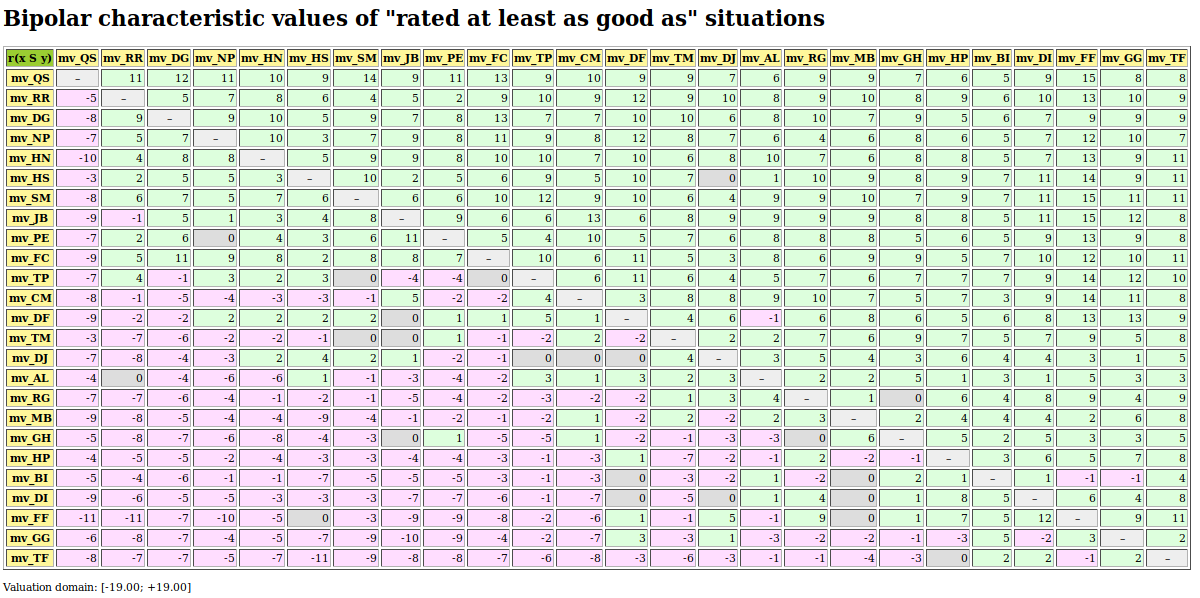
\includegraphics[width=12cm]{Figures/graffiti07_3.png}
\caption{Pairwise majority margins of ``\emph{at least as well rated as}'' rating opinions}
\label{fig:16.4}       % Give a unique label
\end{figure}

Positive characteristic values, validating a global ``\emph{at least as well rated as}'' opinion are marked in light green (see Fig. \ref{fig:16.4}). Whereas negative characteristic values, invalidating such a global opinion, are marked in light red. We may by the way notice that the best-ranked movie 'mv\_QS' is indeed a \Condorcet winner, i.e. better rated than all the other movies by a $65\%$ majority of critics. This majority may be assessed from the average determinateness of the given bipolar-valued outranking digraph $g$.

\begin{lstlisting}      
>>> print( '%.0f%%' % g.computeDeterminateness(InPercents=True) )
   65%
\end{lstlisting}

Notice also the indeterminate situation we observe, for instance, when comparing movie 'mv\_PE' with movie 'mv\_NP'.

\begin{lstlisting}      
>>> g.showHTMLPairwiseComparison('mv_PE','mv_NP')
\end{lstlisting}
\begin{figure}[h]
%\sidecaption
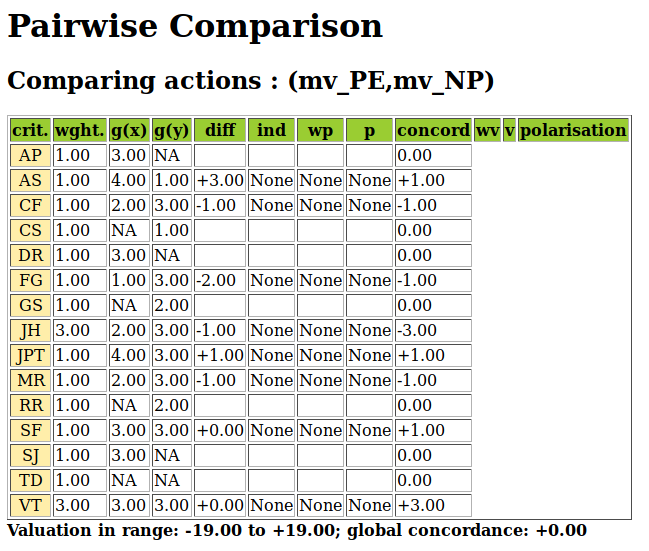
\includegraphics[width=8cm]{Figures/graffiti07_6.png}
\caption{Indeterminate pairwise comparison example.}
\label{fig:16.5}       % Give a unique label
\end{figure}

Only eight, out of the fifteen critics, have seen both movies and the positive opinions do neatly balance the negative ones. A global statement that 'mv\_PE' is ``\emph{at least as well rated as}'' 'mv\_NP'  may in this case hence neither be validated, nor invalidated; a preferential situation that cannot be modelled with any scoring approach.

It is fair, however, to eventually mention here that the \emph{Graffiti} magazine's average scoring method is actually showing a very similar ranking. Indeed, average scores usually confirm well all evident pairwise comparisons, yet \emph{enforce} comparability for all less evident ones.

Notice finally the ordinal correlation \emph{tau} values in Fig. \ref{fig:16.2} 3rd row. Computing these ordinal correlation indexes is the subject of the next Section.
 
\section{\Kendall 's tau index}
\label{sec:16:6}


M. G. Kendall ([KEN-1938p]) defined his ordinal correlation $\tau$ (\emph{tau}) index for linear orders of dimension $n$ as a balancing of the number $Co$ of correctly oriented pairs against the number $In$ of incorrectly oriented pairs. The total number of irreflexive pairs being $n(n-1)$, in the case of linear orders, $Co + In \;=\; n(n-1)$.  Hence $\tau \;=\; \big(\frac{Co}{n(n-1)}\big) \,-\, \big(\frac{In}{n(n-1)}\big)$. In case $In$ is zero, $\tau \;=\; +1$  (all pairs are equivalently oriented); inversely, in case $Co$ is zero, $\tau \;=\; -1$ (all pairs are differently oriented).

Noticing that $\frac{Co}{n(n-1)} \;=\; 1 \,-\, \frac{In}{n(n-1)}$, and recalling that the bipolar-valued negation is operated by changing the sign of the characteristic value, \Kendall 's original \emph{tau} definition implemented in fact the bipolar-valued negation of the non equivalence of two linear orders: 
\begin{equation}
      \tau \;=\; 1 -2\frac{In}{n(n-1)} \;=\; -\big(\,2\frac{In}{n(n-1)} \,-\, 1\,\big) \;=\; 2\frac{Co}{n(n-1)} \,-\, 1,
\end{equation} 
i.e. the normalized majority margin of equivalently oriented irreflexive pairs.

Let $R_1$ and $R_2$ be two random crisp relations defined on a same set of 5 alternatives. We may compute \Kendall 's \emph{tau} index as follows.

\begin{lstlisting}[caption={Computing a relational equivalence digraph},label=list:16.1]
>>> from randomDigraphs import RandomDigraph
>>> R1 = RandomDigraph(order=5,Bipolar=True)
>>> R2 = RandomDigraph(order=5,Bipolar=True)
>>> from digraphs import EquivalenceDigraph
>>> E = EquivalenceDigraph(R1,R2)
>>> E.showRelationTable(ReflexiveTerms=False)
  * ---- Relation Table -----
  r(<=>)|  'a1'	  'a2'	  'a3'	  'a4'	  'a5'	  
  ------|-------------------------------------
   'a1' |    -   -1.00   1.00   -1.00    1.00	 
   'a2' |  -1.00   -    -1.00    1.00   -1.00	 
   'a3' |  -1.00 -1.00    -      1.00    1.00	 
   'a4' |  -1.00  1.00  -1.00     -      1.00	 
   'a5' |  -1.00  1.00  -1.00    1.00     - 	 
   Valuation domain: [-1.00;1.00]
>>> E.correlation
  {'correlation': -0.1, 'determination': 1.0}
\end{lstlisting}
In the table of the equivalence relation $(R_1 \Leftrightarrow R_2)$ above (see Listing \ref{list:16.1} Lines 10-14), we observe that the normalized majority margin of equivalent versus non equivalent irreflexive pairs amounts to $(9 - 11)/20 = -0.1$, i.e. the value of \Kendall 's \emph{tau} index in this plainly determined crisp case (see Line 17).

What happens now with more or less determined and even partially indeterminate relations? May we proceed in a similar way?

\section{Bipolar-valued relational equivalence}
\label{sec:17.2}

Let us now consider two randomly bipolar-valued digraphs $R_1$ and $R_2$ of order five.

\begin{lstlisting}[caption={Two random bipolar-valued digraphs},label=list:16.2]
>>> R1 = RandomValuationDigraph(order=5,seed=1)
>>> R1.showRelationTable(ReflexiveTerms=False)
  * ---- Relation Table -----
   r(R1)|   'a1'   'a2'   'a3'   'a4'   'a5'	  
  ------|------------------------------------
   'a1' |    - 	  -0.66	  0.44	  0.94	-0.84	 
   'a2' |  -0.36    - 	 -0.70	  0.26	 0.94	 
   'a3' |   0.14   0.20	   - 	  0.66	-0.04	 
   'a4' |  -0.48 - 0.76	  0.24	   -  	-0.94	 
   'a5' |  -0.02   0.10	  0.54	  0.94    - 	 
   Valuation domain: [-1.00;1.00]
>>> R2 = RandomValuationDigraph(order=5,seed=2)
>>> R2.showRelationTable(ReflexiveTerms=False)
  * ---- Relation Table -----
   r(R2)|   'a1'   'a2'   'a3'   'a4'   'a5'	  
  ------|-----------------------------------
   'a1' |   -     -0.86  -0.78  -0.80  -0.08	 
   'a2' |  -0.58    -     0.88   0.70  -0.22	 
   'a3' |  -0.36   0.54	   -    -0.46   0.54	 
   'a4' |  -0.92   0.48   0.74    -    -0.60	 
   'a5' |   0.10   0.62   0.00   0.84    - 	 
   Valuation domain: [-1.00;1.00]
\end{lstlisting}

We may notice in the relation tables shown above that 9 pairs, like (a1,a2) or (a3,a2) for instance, appear equivalently oriented (see Listing \ref{list:16.2} Lines 6,17 or 8,19). The \texttt{EquivalenceDigraph} class implements this relational equivalence relation between digraphs $R_1$ and $R_2$ (see Listing \ref{list:16.3}).
\begin{lstlisting}[caption={Bipolar-valued Equivalence Digraph},label=list:16.3]
>>> eq = EquivalenceDigraph(R1,R2)
>>> eq.showRelationTable(ReflexiveTerms=False)
  * ---- Relation Table -----
   r(<=>)|  'a1'  'a2'   'a3'   'a4'   'a5'	  
   ------|---------------------------------
   'a1' |   - 	  0.66  -0.44  -0.80   0.08	 
    'a2' |  0.36   -    -0.70   0.26  -0.22	 
    'a3' | -0.14  0.20    -    -0.46  -0.04	 
    'a4' |  0.48 -0.48   0.24    -     0.60	 
    'a5' | -0.02  0.10   0.00   0.84    - 	 
   Valuation domain: [-1.00;1.00]
\end{lstlisting}

In our bipolar-valued epistemic logic, logical disjunctions and conjunctions are implemented as $\max$, respectively $\min$ operators. Notice also that the logical equivalence $(R_1 \Leftrightarrow R_2)$ corresponds to a double implication $(R_1 \Rightarrow R_2)\, \wedge \, (R_2 \Rightarrow  R_1)$ and that the implication $(R_1 \Rightarrow R_2)$ is logically equivalent to the disjunction $(\neg R_1 \vee R_2)$.

When $r(x\,R_1\, y)$ and $r(x\,R_2\; y)$ denote the bipolar-valued characteristic values of relation $R_1$, resp. $R_2$, we may hence compute as follows a majority margin $M(R_1 \Leftrightarrow R_2)$ between equivalently and not equivalently oriented irreflexive pairs $(x,y)$.
\begin{equation}\label{eq:16:2}
\left.\begin{aligned}
M(R_1 \Leftrightarrow R_2) \; &= \\  &\sum_{(x \neq y)} \Big[ \min \Big( \max \big( -r(x \,R_1\, y), r(x \,R_2\, y)\big), \max \big( -r(x \,R_2\, y), r(x \,R_1\, y)\big) \Big) \Big]\;.
\end{aligned}\right.
\end{equation}

$M(R_1 \Leftrightarrow R_2)$ is thus given by the sum of the non reflexive terms of the relation table of $eq$, the relation equivalence digraph computed above (see Listing \ref{list:16.3}).

In the crisp case, $M(R_1 \Leftrightarrow R_2)$  is now normalized with the maximum number of possible irreflexive pairs, namely $n(n-1)$. In a generalized $r$-valued case, the maximal possible equivalence majority margin $M$ corresponds to the sum $D$ of the conjoint determinations of $(x \,R_1\, y)$ and $(x \,R2\, y)$ (see [BIS-2012p]). 
\begin{equation}
  D \;=\; \sum_{x \neq y} \min \Big[ abs\big(r(x \,R_1\, y) \big), abs \big( r(x \,R_2\, y \big)  \Big]\;.
\end{equation}
Thus, we obtain in the general $r$ -valued case:
\begin{equation}
  \tau(R_1,R_2) \;=\; \frac{M(R_1 \Leftrightarrow R_2)}{D}\;.
\end{equation}

$\tau(R_1,R_2)$ corresponds thus to a classical ordinal correlation index, but restricted to the conjointly determined parts of the given relations $R_1$ and $R_2$. In the limit case of two crisp linear orders, $D$ equals $n(n-1)$, i.e. the number of irreflexive pairs, and we recover hence \Kendall 's original \emph{tau} index definition.

It is worthwhile noticing that the ordinal correlation index $\tau(R_1,R_2)$ we obtain above corresponds to the ratio of
\begin{itemize}
\item $r(R_1 \Leftrightarrow R_2) \;=\; \frac{M(R_1 \Leftrightarrow R_2)}{n(n-1)}$: the normalized majority margin of the pairwise \emph{relational} equivalence statements, also called \emph{valued ordinal correlation}, and 
\item $d \;=\; \frac{D}{n(n-1)}$ : the normalized determination of the corresponding pairwise relational equivalence statements, in fact the \emph{determinateness} of the relational equivalence digraph.
\end{itemize}

We have thus successfully \emph{out-factored} the epistemic determination effect from the ordinal correlation effect. With completely determined relations, $\tau(R_1,R_2) \;=\; r(R_1 \Leftrightarrow R_2)$. By convention, we set the ordinal correlation with a completely indeterminate relation, i.e. when $D = 0$, to the indeterminate correlation value $0.0$. With uniformly chosen random $r$-valued relations, the expected $\tau$ index is $0.0$, denoting in fact an indeterminate correlation. The corresponding expected normalized determination $d$ is about $0.333$ (see [BIS-2012p]).

We may verify these relations with help of the corresponding equivalence digraph $eq$ (see Listing \ref{list:16.4}).

\begin{lstlisting}[caption={Computing the ordinal correlation index from the equivalence digraph},label=list:16.4]
>>> eq = EquivalenceDigraph(R1,R2)
>>> M = Decimal('0'); D = Decimal('0')
>>> n2 = eq.order*(eq.order - 1)
>>> for x in eq.actions:
...     for y in eq.actions:
...         M += eq.relation[x][y]
...         D += abs(eq.relation[x][y])
>>> print('r(R1<=>R2) = %+.3f, d = %.3f, tau = %+.3f' % (M/n2,D/n2,M/D))   
  r(R1<=>R2) = +0.026, d = 0.356, tau = +0.073  
\end{lstlisting}

In general we simply use the \texttt{computeOrdinalCorrelation()} method which renders a dictionary with a \texttt{correlation} ($\tau$) and a \texttt{determination} ($d$) attribute. We may recover $r(\Leftrightarrow)$ by multiplying $\tau$ with $d$ (see Listing \ref{list:16.5} Line 4). 

\begin{lstlisting}[caption={Directly computing the ordinal correlation index},label=list:16.5]
>>> corrR1R2 = R1.computeOrdinalCorrelation(R2)
>>> tau = corrR1R2['correlation']
>>> d = corrR1R2['determination']
>>> r = tau * d
>>> print('tau(R1,R2) = %+.3f, d = %.3f,\
...        r(R1<=>R2) = %+.3f' % (tau, d, r))
  tau(R1,R2) = +0.073, d = 0.356, r(R1<=>R2) = +0.026
\end{lstlisting}

We provide for convenience a direct \texttt{showCorrelation} method:

\begin{lstlisting}
>>> corrR1R2 = R1.computeOrdinalCorrelation(R2)
>>> R1.showCorrelation(corrR1R2)
  Correlation indexes:
    Extended Kendall tau       : +0.073
    Epistemic determination    :  0.356
    Bipolar-valued equivalence : +0.026
\end{lstlisting}

We may now illustrate the quality of the global ranking of the movies shown with the heat map in Fig. \ref{fig:16.2}. 

\section{Fitness of ranking heuristics}
\label{sec:16.3}

We reconsider the bipolar-valued outranking digraph $g$ modelling the pairwise global ``\emph{at least as well rated as}'' relation among the 25 movies seen above.

\begin{lstlisting}[caption={Global movies outranking digraph},label=list:16.6]
>>> g = BipolarOutrankingDigraph(t,Normalized=True)
  *------- Object instance description ------*
   Instance class   : BipolarOutrankingDigraph
   Instance name    : rel_grafittiPerfTab.xml
   Actions          : 25
   Criteria         : 15
   Size             : 390
   Determinateness  : 65%
   Valuation domain : {'min': Decimal('-1.0'),
                       'med': Decimal('0.0'),
                       'max': Decimal('1.0'),}
>>> g.computeCoSize()
  188
\end{lstlisting}

Out of the $25 \times 24 = 600$ irreflexive movie pairs, digraph $g$ contains 390 positively validated, 188 positively invalidated, and 22 indeterminate outranking situations (see the zero-valued cells in Fig. \ref{fig:16.4}).

Let us now compute the normalized majority margin $r(\Leftrightarrow)$  of the equivalence between the marginal critic's pairwise ratings and the global \NetFlows ranking shown in the ordered heat map (see Fig. \ref{fig:16.2}).

\begin{lstlisting}[caption={Computing marginal criterion correlations with global \NetFlows ranking},label=list:16.7]
>>> from linearOrders import NetFlowsOrder
>>> nf = NetFlowsOrder(g)
>>> nf.netFlowsRanking
  ['mv_QS', 'mv_RR', 'mv_DG', 'mv_NP', 'mv_HN', 'mv_HS', 'mv_SM',
   'mv_JB', 'mv_PE', 'mv_FC', 'mv_TP', 'mv_CM', 'mv_DF', 'mv_TM',
   'mv_DJ', 'mv_AL', 'mv_RG', 'mv_MB', 'mv_GH', 'mv_HP', 'mv_BI',
   'mv_DI', 'mv_FF', 'mv_GG', 'mv_TF']
>>> for i,item in enumerate(\
...       g.computeMarginalVersusGlobalRankingCorrelations(\
...              nf.netFlowsRanking,ValuedCorrelation=True) ):\
...     print('r(%s<=>nf) = %+.3f' % (item[1],item[0]) )   

  r(JH<=>nf)  = +0.500
  r(JPT<=>nf) = +0.430
  r(AP<=>nf)  = +0.323
  r(DR<=>nf)  = +0.263
  r(MR<=>nf)  = +0.247
  r(VT<=>nf)  = +0.227
  r(GS<=>nf)  = +0.160
  r(CS<=>nf)  = +0.140
  r(SJ<=>nf)  = +0.137
  r(RR<=>nf)  = +0.133
  r(TD<=>nf)  = +0.110
  r(CF<=>nf)  = +0.110
  r(SF<=>nf)  = +0.103
  r(AS<=>nf)  = +0.080
  r(FG<=>nf)  = +0.027
\end{lstlisting}

In Listing \ref{list:16.7} (see Lines 13-27), we recover the relational equivalence characteristic values shown in the third row of the table in Fig. \ref{fig.16.2}. The global \NetFlows ranking represents obviously a rather balanced compromise with respect to all movie critics' opinions as there appears no valued negative correlation with anyone of them. The \NetFlows ranking apparently takes also correctly in account that the journalist $JH$, a locally renowned movie critic, shows a higher significance weight (see Line 13).

The ordinal correlation between the global \NetFlows ranking and the digraph $g$ may be furthermore computed as follows: 

\begin{lstlisting}[caption={Computing correlation between \NetFlows and global outranking },label=list:16.8]
>>> corrgnf = g.computeOrdinalCorrelation(nf)
>>> g.showCorrelation(corrgnf)
  Correlation indexes:
    Extended Kendall tau       : +0.780
    Epistemic determination    :  0.300
    Bipolar-valued equivalence : +0.234
\end{lstlisting}

We notice in Listing \ref{List:16.8} Line 4 that the ordinal correlation $\tau(g,nf)$ index between the \NetFlows ranking $nf$ and the determined part of the outranking digraph $g$ is quite high ($+0.78$). Due to the rather high number of missing data, the $r$ -valued relational equivalence between the $nf$ and the $g$ digraph, with a characteristics value of only $+0.234$, may be misleading. Yet, $+0.234$ still corresponds to a $62\%$ majority support of nthe movie critics' rating opinions.

It would be interesting to compare similarly the correlations one may obtain with other global ranking heuristics, like the \Copeland.

\section{Illustrating preference divergences}
\label{sec:16.4}

The valued relational equivalence index gives us a further measure for studying how \emph{divergent} appear the rating opinions expressed by the movie critics.
\begin{figure}[h]
\sidecaption
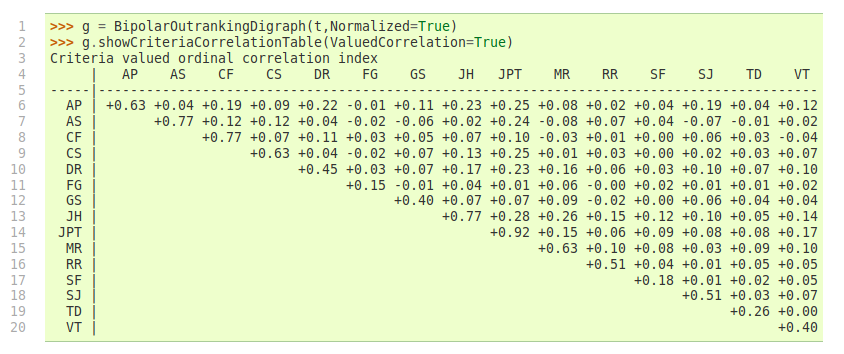
\includegraphics[width=12cm]{Figures/correlationTable.png}
\caption{Pairwise valued correlation of movie critics.} 
\label{fig:16.6}       % Give a unique label
\end{figure}

It is remarkable to notice here that, due to the quite numerous missing data, all pairwise valued ordinal correlation indexes $r(x\Leftrightarrow y)$ appear to be of low value, except the diagonal ones. These reflexive indexes $r(x\Leftrightarrow x)$ would trivially all amount to $+1.0$ in a plainly determined case. Here they indicate a reflexive normalized determination score $d$, i.e. the proportion of pairs of movies each critic did evaluate. Critic 'JPT' (the editor of the Graffiti magazine), for instance, evaluated all but one ($d = 24\times23/600 = 0.92$), whereas critic 'FG' evaluated only 10 movies among the 25 in discussion ($d = 10\times9/600 = 0.15$).

To get a picture of the actual divergence of rating opinions concerning jointly seen pairs of movies, we may develop a Principal Component Analysis of the corresponding $\tau$ correlation matrix\footnote{The 3D PCA plot method requires a running R statistics software  (https://www.r-project.org/) installation and the Calmat matrix calculator (see the \texttt{calmat} directory in the \Digraph resources)}. The 3D plot of the first 3 principal axes is shown in Fig. \ref{fig:16.2}.

\begin{lstlisting}
>>> g.export3DplotOfCriteriaCorrelation(ValuedCorrelation=False)
\end{lstlisting}
\begin{figure}[h]
%\sidecaption
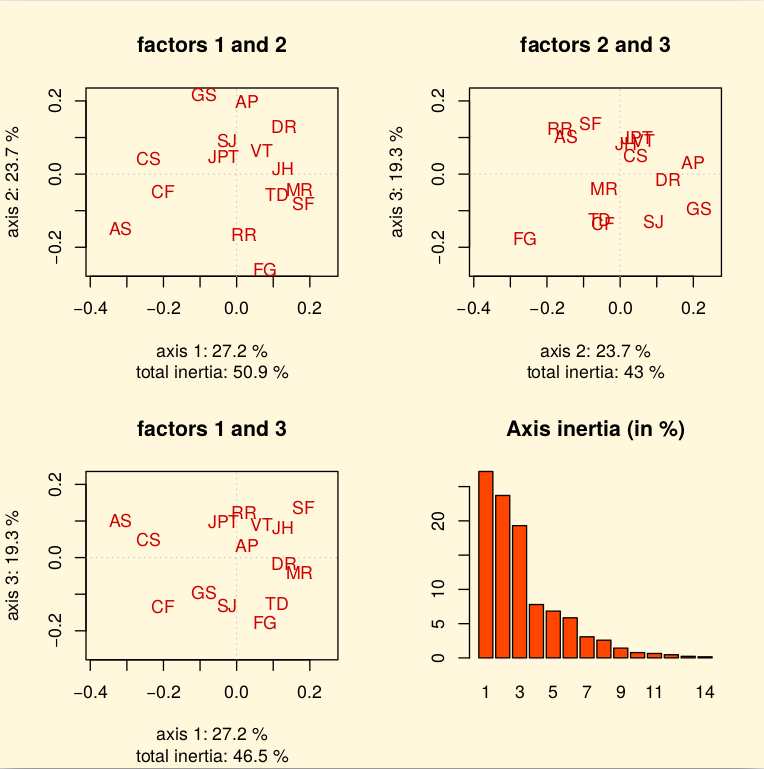
\includegraphics[width=10cm]{Figures/correlationPCA.png}
\caption{3D PCA plot of the criteria ordinal correlation matrix.}
\label{fig:16.7}       % Give a unique label
\end{figure}
The first 3 principal axes support together about $70\%$ of the total inertia. Most eccentric and opposed in their respective rating opinions appear, on the first principal axis with $27.2\%$ inertia, the conservative daily press against labour and public press. On the second principal axis with $23.7.7\%$ inertia, it is the people press versus the cultural critical press. And, on the third axis with still $19.3\%$ inertia, the written media appear most opposed to the radio media.

\section{Exploring the ``\emph{better rated}''  and the ``\emph{as well as rated}'' opinions}
\label{sec:16.5}

In order to furthermore study the quality of a ranking result, it may be interesting to have a separate view on the asymmetric and symmetric parts of the ``\emph{at least as well rated as}'' opinions (see Section \ref{sec:2.3}).

Let us first have a look at the pairwise asymmetric part, namely the ``\emph{better rated than}'' and ``\emph{less well rated than}'' opinions of the movie critics. 

\begin{lstlisting}
>>> from digraphs import AsymmetricPartialDigraph
>>> ag = AsymmetricPartialDigraph(g)
>>> ag.showHTMLRelationTable(\
...    actionsList=g.computeNetFlowsRanking(),ndigits=0)
\end{lstlisting}
\begin{figure}[h]
%\sidecaption
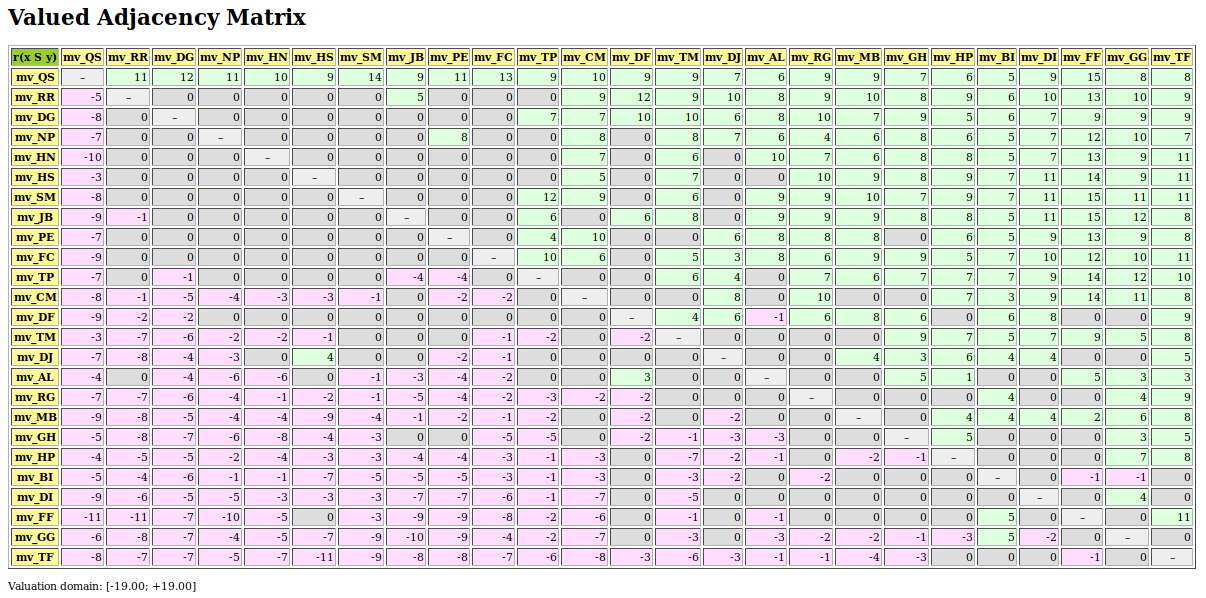
\includegraphics[width=12cm]{Figures/asymmetricPart.png}
\caption{Asymmetric part of \emph{graffiti07} digraph}
\label{fig:16.8}       % Give a unique label
\end{figure}
We notice here that the \NetFlows ranking rule inverts in fact just three ``\emph{less well rated than}'' opinions and four ``\emph{better rated than}'' ones. A similar look at the symmetric part, the pairwise ``\emph{as well rated as}'' opinions, suggests a preordered preference structure in several equivalently rated classes.

\begin{lstlisting}
>>> from digraphs import SymmetricPartialDigraph
>>> sg = SymmetricPartialDigraph(g)
>>> sg.showHTMLRelationTable(\
...          actionsList=g.computeNetFlowsRanking(),\
...          ndigits=0)
\end{lstlisting}
\begin{figure}[h]
%\sidecaption
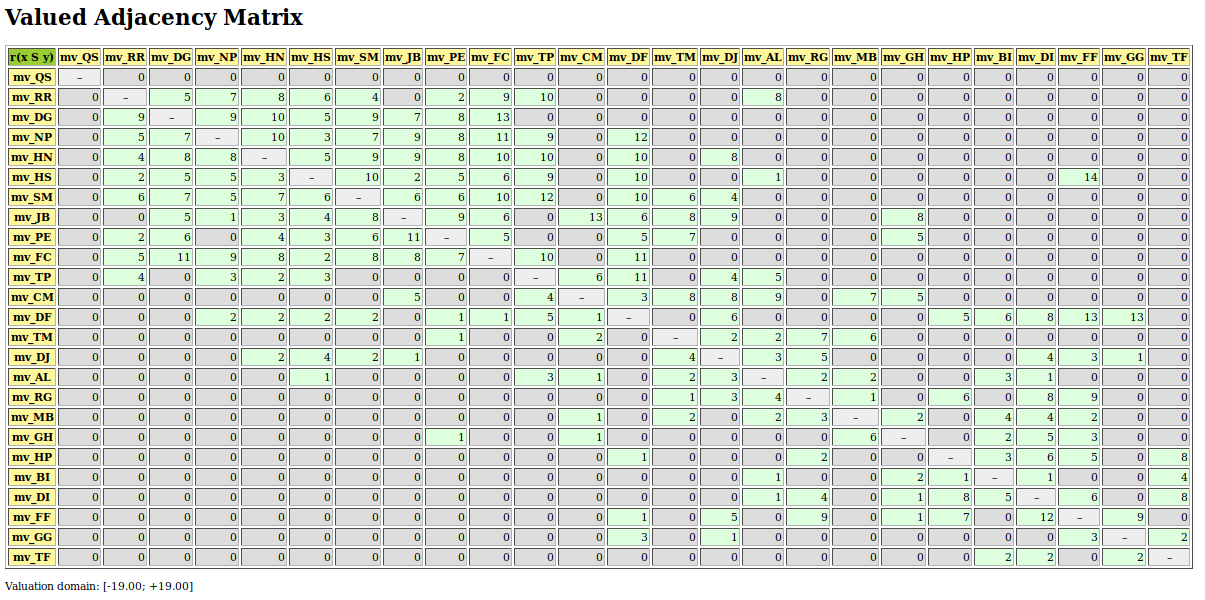
\includegraphics[width=12cm]{Figures/symmetricPart.png}
\caption{Symmetric part of \emph{graffiti07} digraph}
\label{fig:16.9}       % Give a unique label
\end{figure}
Such a preordering of the movies may, for instance, be computed with the \texttt{computeRankingByChoosing()} method, where we iteratively extract dominant kernels --best remaining choices-- and absorbent kernels --worst remaining choices-- (see the next Chapter). We operate therefore on the asymmetric ``\emph{better rated than}'' opinions, i.e. the codual of the ``\emph{at least as well rated as}'' opinions \footnote{A kernel in a digraph $g$ is a clique in the dual digraph $-g$.} (see Listing \ref{list:16.9} Line 2).

\begin{lstlisting}[caption={Bipolar ranking-by-choosing the Grafitti movies},label=list:16.9]
>>> from transitiveDigraphs import RankingByChoosingDigraph
>>> rbc = RankingByChoosingDigraph(g,CoDual=True)
>>> rbc.showRankingByChoosing()
  Ranking by Choosing and Rejecting
    1st Best Choice ['mv_QS']
      2nd Best Choice ['mv_DG','mv_FC','mv_HN','mv_HS','mv_NP',
                       'mv_PE','mv_RR','mv_SM']
	3rd Best Choice ['mv_CM','mv_JB','mv_TM']
          4th Best Choice ['mv_AL','mv_TP']
          4th Worst Choice ['mv_AL','mv_TP']
        3rd Worst Choice ['mv_GH','mv_MB','mv_RG']
      2nd Worst Choice ['mv_DF','mv_DJ','mv_FF','mv_GG']
    1st Worst Choice ['mv_BI','mv_DI','mv_HP','mv_TF']
\end{lstlisting}

In the next Chapter \ref{sec:17}, we thouroughly discuss the computation of kernels in bipolar-valued digraphs.
